\chapter{Methodology}
\label{ch_methodology}

%This is what I did to test and confirm my hypothesis.


%You may want to split this chapter into sub chapters depending on your design. I suggest you change
%the title to something more specific to your project.

%This is where you describe your design process in detail, from component/device selection to actual
%design implementation, to how you tested your system. Remember detail is important in technical
%writing. Do not just write I used a computer give the computer specifications or the oscilloscopes part
%number. Describe the system in enough detail so that someone else can replicate your design as well
%as your testing methodology.

%If you use or design code for your system, represent it as flow diagrams in text.

\section{Outline}

This study set out to investigate the performance of modules created for a uni-directional data link in the context of laser tag systems. The following chapter presents the methodology that was followed throughout the investigation. A phased approach was taken and the following chapter gives a break down of those phases.

\begin{figure}[H]
	\centering
	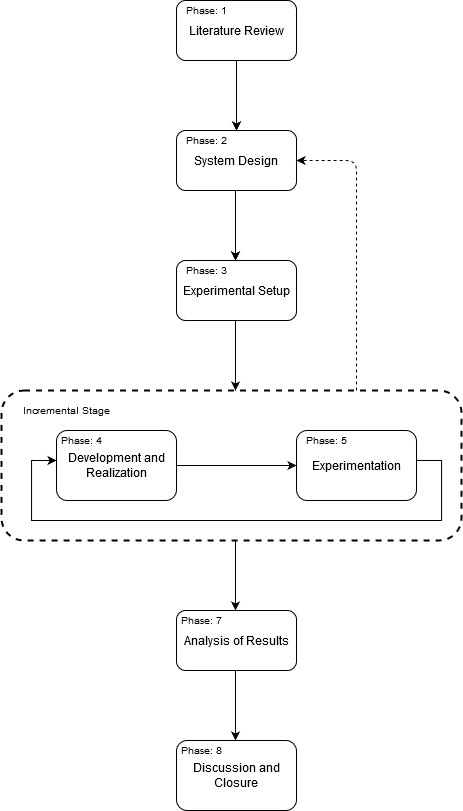
\includegraphics[width=0.5\textwidth]{figures/methodology/methodology}
	\caption{Methodology Flow Diagram}
	\label{fig:methodology_overview}
\end{figure}

%todo: this will need re-wroking after finilized the flow diagram
The first phase involves investigating the relevant literature. The second phase involves identifying and designing the modular subsystems, this phase of the project incorporates a portion of feedback from the incremental stage. The third phase is the experimental setup during which experiments are devised and test/measurement equipment selected. Following the experimental setup is an iterative stage which comprises phase four and five. During phase four the modules are developed according to the designs produced in the second phase. Phase five then involves performing the experiments devised in the third phase to evaluate the modules.

The experimentation phase loops back to the development stage illustrating that some experiments were performed progressively as modules are realized. Following the design paradigm of the spiral model, a feedback path from the incremental stage back to the design exists to illustrated that certain design choices were made based on the experimental results.

During phase 7 the results are compiled and analysed. During the 8\textsuperscript{th} phase these results are interpreted and conclusions are drawn bringing closure to the research project.


%todo: the following sections are very 'outdated'/incomplete
\section{Phase 1 - Literature}

During the first phase of the project, the relevant literature is reviewed. The objective of this phase is to determine the various techniques that have been established in the field of optical communication. For each of the topics a broad overview is presented, followed by a detailed review of specific concepts and theories.

The design and evaluation of a complex communication system involves reviewing theory in various areas and the following questions served as a guide for surveying the available literature.

%todo: consider improving these questions
\begin{itemize}
	%\item What are current examples of uni-directional communication systems?
	\item How might non-laser light be focused into a narrow beam? %Optics
	\item What properties make infrared light useful? %Optics
	\item What methods exist for detection of light? %Detection of Raditation
	\item What techniques exist for reliable communication? %Reliable Communication
	\item What techniques exist for the purpose of tone detection? %DSP &Analog processing
	%an item on filtering and pre-dsp stuff?
\end{itemize}

The literature review is presented in chapter \ref{ch_literature}.

%%%%%%%%%%%%%%%%%%%%

\section{Phase 2 - Design}

The design phase of this investigation is dedicated to the development of the individual modules and software algorithms. This phase begins with a decomposition of the uni-directional communication system into a set of modules. Figure \ref{fig:designoverview} provides a high-level overview of the system decomposition.

\begin{figure}[H]
	\centering
	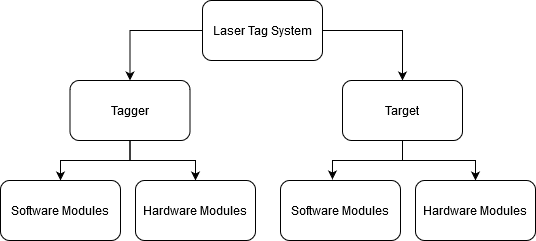
\includegraphics[width=0.7\linewidth]{figures/methodology/design_overview}
	\caption{Design Overview}
	\label{fig:designoverview}
\end{figure}

The second phase is documented in chapter \ref{ch_design}. For each module a brief description of the purpose and required functionality of the module is given. The design of module is then presented, including important calculations, circuit schematics and relevant diagrams where appropriate. For each module an image of the final implementation is also shown.

Throughout the design phase, various simulations were used to predict the behaviour of algorithms\footnote{Octave was used to validate algorithms} and circuits\footnote{LTSpice was used to simulate circuits}.

%%%%%%%%%%%%%%%%%%%%

\section{Phase 3 - Development and Realization}

The third phase concerns the development of the individual modules. During this phase each module was realized according its design.

Modules were first implemented on a breadboard to confirm valid behaviour. In the case of a failed implementation due to a design oversight the design was reworked, this is illustrated using a dotted feedback path from phase 3 to phase 2 in figure \ref{fig:methodology_overview}. Only the final module design and implementation has been documented in the body of this report.

With the exception of the STM32 development boards, all the module designs were implemented on strip-board. The use of PCB was avoided due to uncertainty caused by the COVID-19 epidemic.

%%%%%%%%%%%%%%%%%%%%


\section{Phase 4 - Experimental Setup}

The fourth phase is the experimental set-up. This phase outlines the procedure followed using test and measurement equipment along with a module or collection of modules for the purposes of gathering performance data.

Due to the unique functionality of each module, it is necessary to use different experimental setups to evaluate different modules. Hence phase four forms part of an \textit{iterative stage} which is used to illustrate that for various phases of experimentation, a unique experimental setup has been devised.


%%%%%%%%%%%%%%%%%%%%



\section{Phase 5 - Experimentation}
%Experimentation will achieve two goals, validation/verification and performance testing.

The experimentation phase has two objectives. It sets out to confirm the expected performance of system modules and determine through empirical analysis specifications for hardware and software components.

Experiments will involve either comparing measured results to theoretical or simulated results and it evaluates the performance of system modules by determining 



\section{Phase 7 - Analysis of Results}



\section{Phase 8 - Discussion and Closure}








